\newpage
\noindent \begin{minipage}{\linewidth}
Inoltre notiamo che la fase non è quella tipica del filtro notch già studiato nella precedente esperienza. Questo è dovuto al fatto che noi abbiamo considerato la differenza di fase tra i due segnali ai capi del ponte di Wien, non tra segnale in input e differenza dei due segnali in output. Tale relazione risulta infatti essere:

\begin{equation}
\vartheta_{out|in}=arctan\left[\frac{2 C R \omega \left(C^2 R^2 \omega^2-1\right)}{C^4 R^4 \omega^4+C^2 R^2 \omega^2+1}\right]
\label{teo}
\end{equation}

Poichè non è stata rilevata la differenza di fase direttamente durante l'esperienza, essa è stata calcolata dai dati sperimentali imponendo la condizione, valida per ogni $t$:

\begin{equation}
V_{out}sin(\omega t + \vartheta)=V(CH1)sin(\omega t + \varphi)-V(CH2)sin(\omega t)
\end{equation}

Scegliendo come tempo $t=0$, e applicando un arcoseno, otteniamo subito lo sfasamento del segnale in uscita rispetto a quello in entrata.

\begin{equation}
\vartheta=asin\left(\frac{V(CH1)}{V_{out}}sin(\varphi)\right)
\label{dati}
\end{equation}


Riportiamo in Fig \ref{fig:pahser} la legge teorica (\ref{teo}) e dati sperimentali rielaborati attraverso (\ref{dati}). Nonostante la propagazione degli errori, nel grafico non sono ancora distinguibili le barre d'errore.
\end{minipage}

% questa dovrebbe essere la fase GIUSTA (da mettere a parte) y=180/pi*np.arctan((2*C*R*w*(-1 + (C*R*w)**2))/(1 + (C*R*w)**2 + (C*R*w)**4))

\section{Conclusioni}
\noindent \begin{minipage}{\linewidth}
Attraverso il ponte di Wien siamo riusciti ad ottenere una misura precisa del valore di un capacitore incognito. Un valore compatibile con quello misurato dal multimetro e dichiarato dal costruttore è ottenibile sia dalle equazioni di bilanciamento che dalla loro combinazione. Notiamo dai dati riportati in tabella che quest'ultimo procedimento è quello che permette una stima affetta da minor errore. 
Abbiamo verificato il funzionamento del ponte di Wien come filtro notch. Esso, come già detto, non risulta efficace come un filtro notch costruito utilizzando capacitore in serie ad un'induttanza. Inoltre, per le scelte da noi fatte di resistenze e capacità, l'intensità picco-picco del segnale in output non potrà mai essere superiore a $\frac{V_{in}}{2}$.
\end{minipage}

\begin{figure}[H]%[30]
	\centering
	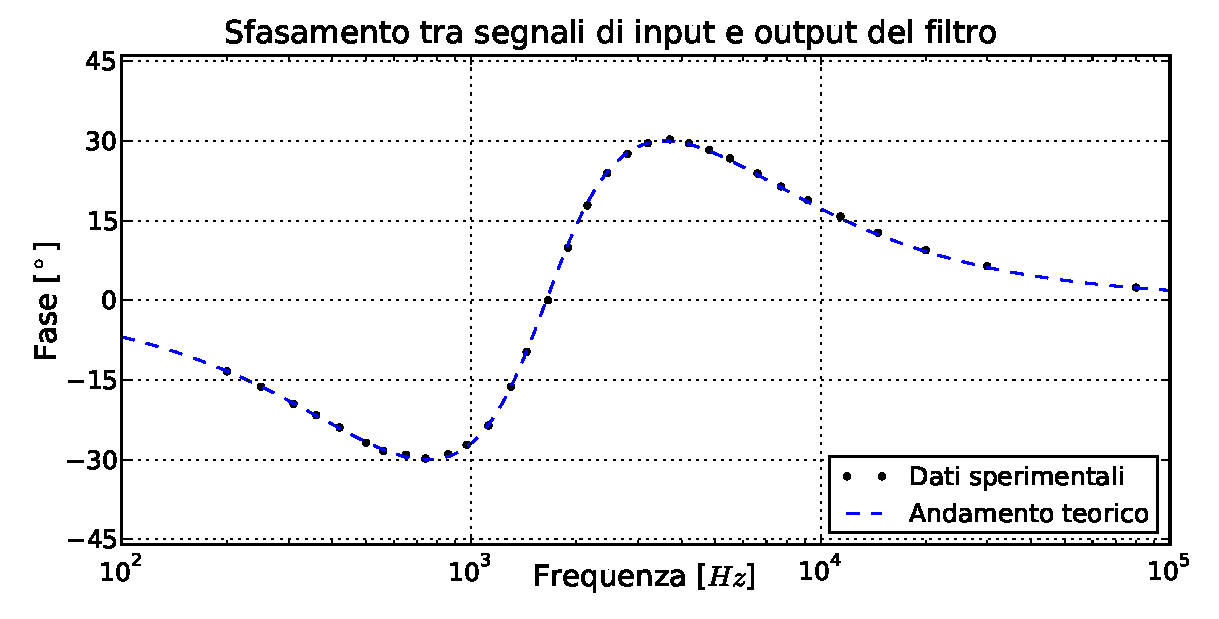
\includegraphics[width=150mm]{i_peli.pdf}
		\caption{Nel grafico sono riportati i valori di differenza di fase tra il segnale in input al circuito e il segnale in output. Ricordiamo che i dati sperimentali sono stati rielaborati usando la formula (\ref{dati}).}
	\label{fig:pahser}
\end{figure}